\chapter{Overview}

The goal of this thesis is to implement a simple compiler for a subset of TypeScript. This chapter describes the high-level architecture of the compiler, and related technologies used or considered for its implementation.


\section{Requirements}

The proposed compiler will be primarily used in resource constrained environments such as microcontrollers or single board computers. For this reason, the compiler must be small and resource efficient. It will be used as a part of the JavaScript runtime Jaculus (described in Section \ref{jaculus}).

Because the compiler should be simple, it will only perform compilation of selected parts of the input program. After compilation is completed, it will not do any further work during the execution of a program. The compilation will be performed at the level of individual functions. If multiple suitable functions are found in a single file, they will be compiled together and statically linked.

The compiler must be able to compile a subset of TypeScript that will make it possible to write useful subroutines which can make use of the increased performance of compiled code. Initially, the compiler will support only a small part of the language, but it should be possible to extend in the future.

Examples of programs that should be able to take advantage of the compiler are:
\begin{itemize}
    \item computational functions,
    \item functions for graphical rendering,
    \item inner computations of more complex functions.
\end{itemize}


\section{Architecture}

The compiler is consists of multiple parts, each of which is responsible for a single step of the compilation process. The compiler is designed to depend on external libraries as weakly as possible. This means that it is possible to replace these libraries with other implementations without an extensive rewrite of the compiler (particularly the compiler backend MIR, and the JavaScript engine QuickJS).

An overview of the architecture of the compiler is shown in Figure \ref{fig:architecture}.

\begin{figure}
    \centering
    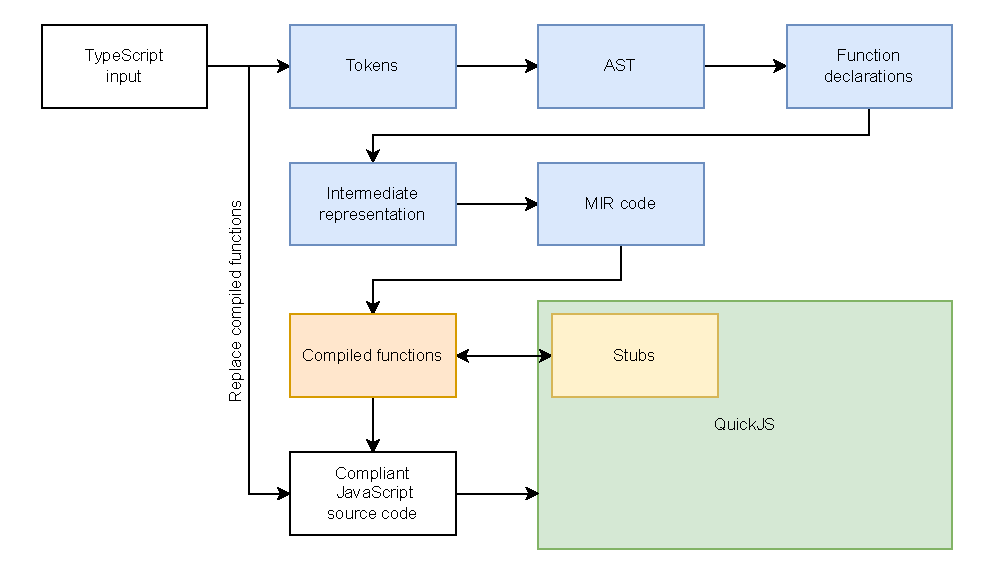
\includegraphics[width=\textwidth, draft=false]{assets/img/architecture.pdf}
    \caption{Architecture of the compiler.}
    \label{fig:architecture}
\end{figure}


\section{Jaculus}\label{jaculus}

Jaculus~\cite{jaculusthesis} is a platform for programming microcontrollers using JavaScript. It is divided into multiple libraries. The core library, \textit{Jaculus-machine}, provides a JavaScript runtime environment based on the QuickJS JavaScript engine~\cite{quickjs}, and implements a set of C++ abstractions around it. It also provides some core features for the runtime, such as an event loop\footnote{An event loop is a construct that realizes processing of events. Their processing is performed sequentially.} or libraries available in the JavaScript environment. Jaculus-machine can be used independently of the rest of Jaculus -- for example for embedding into other applications.

Other Jaculus libraries realize communication between a JavaScript runtime running on a microcontroller and a host computer used by the programmer (e.g., for uploading new programs), and provide platform-specific libraries for using the peripherals of the microcontroller.

This thesis focuses on extending the Jaculus-machine library with an ahead-of-time compiler for a subset of TypeScript.


\section{QuickJS}

QuickJS \cite{quickjs} is an embeddable JavaScript engine created by Fabrice Bellard and other contributors. The current version, which is used in Jaculus-machine, implements the ECMAScript 2023 Language Specification~\cite{ecma262}.

QuickJS is designed to have small code and memory footprint, and to be easily embeddable in larger programs. An important goal of QuickJS is having a very fast startup time.

QuickJS uses a stack-based bytecode machine. To shorten its startup time, QuickJS generates bytecode while parsing the source code without the use of an intermediate representation or an AST. Some simple optimizations are then performed on the generated bytecode.


\section{Compiler backends}

For the implementation of our compiler, we have chosen to use an existing compiler backend. This section describes several compiler backends that were considered.

We need the backend to be reasonably small and fast -- it should be able to compile reasonably large programs with 2 MB of memory available. It needs to be usable as a library, and its input should be a platform independent intermediate representation of the program. It should also handle register allocation.

Preferably, we would like the backend to support 32-bit architectures, especially Xtensa and riscv32. These two architectures are used in microcontroller series ESP32, which is the primary target platform for Jaculus.

While none of the choices is ideal, we have ultimately chosen the MIR compiler backend which suites our needs the best.


\subsection{MIR}

MIR~\cite{mir} is a backend designed for use in JIT compilers. Its input is a statically typed, platform independent intermediate representation. MIR supports multiple architectures -- amd64, aarch64, ppc64le, s390x, and riscv64. It should also be possible to implement support for other architectures, including 32-bit ones. MIR implements several optimization passes.

MIR provides an API for generating its intermediate representation. The output of the backend are pointers to the generated code (functions) which can be called directly using the calling convention native to current platform.

MIR code uses an unlimited number of \textit{local variables} which may be used as operands for instructions. They can have one of the following types -- 64-bit integer, float, double, or long double. While the choice is natural on 64-bit targets, it will make porting the backend to 32-bit architectures more difficult.


\subsection{Cwerg BE}

Cwerg backend is primarily developed in conjunction with the Cwerg language~\cite{cwerg}. The focus of the project is to keep a small, maintainable codebase with less focus on code performance.

Similarly to MIR, Cwerg provides an API for generating its intermediate representation. Functions in the generated machine code can be called using the calling convention native to current platform.

The author of Cwerg advertises the backend to be suitable for use in JIT compilers. However, because the backend stores its in global data structures, which are not reset after compilation, it can be only used as a one-time, ahead-of-time compiler. This behavior makes it unsuitable for our use case because we want to be able to reset the runtime (and thus perform a new compilation) multiple times during the execution of a single process.


\subsection{LLVM}

LLVM~\cite{llvm} is a standard consideration when implementing a compiler thanks to its extensive feature set and list of supported platforms. Because of its size, however, it has large hardware requirements and slow startup time. It is therefore infeasible to use in constrained environments.


\subsection{DynASM}

DynASM~\cite{dynasm} is a JIT library primarily used in the LuaJIT project. DynASM by itself is retargetable to other languages, however, it is still strongly tied with the Lua world. The preprocessing of input text for DynASM is implemented in Lua and an interpreter for Lua is therefore required to use DynASM.

For the use in constrained environments, having a second interpreter is not ideal.


\subsection{QBE}

QBE~\cite{qbe} is a small compiler backend with a focus on simplicity and small code size. It is not designed as a library but as a standalone compiler. While it is possible to modify QBE to be usable directly from a program, another limitation is that the input of QBE is a text program. QBE also generates text assembly as its output, which has to be assembled by an external assembler. The backend supports amd64, arm64, and riscv64 architectures.


\subsection{Eigen Compiler Suite}

Eigen Compiler Suite~\cite{ecs} is a full compiler for several languages with support for multiple architectures. It is primarily designed as a standalone compiler, however, it is written in a way that makes it convenient to use its individual parts as a library.

Internally, the compiler uses a platform independent intermediate representation, and the compiler backend can be used independently. It supports many architectures, including amd64, aarch32, aarch64, AVR or Xtensa.

An unfortunate downside of the compiler is that it implements a custom calling convention which makes it difficult to interface with the compiled functions. The compiler also does not generate particularly efficient code, especially for less common architectures such as Xtensa.
